\documentclass[11pt,a4paper]{article}
\usepackage{fontspec}
\setmainfont{cmunrm.otf}[BoldFont=cmunbx.otf,ItalicFont=cmunti.otf,BoldItalicFont=cmunbi.otf]
\setmonofont{cmuntt.otf}[BoldFont=cmuntb.otf]
\usepackage[russian]{babel}
\usepackage[margin=23mm]{geometry}
\usepackage{amsmath,amssymb,array,booktabs,tabularx,graphicx,fancyvrb,caption,hyperref}
\hypersetup{hidelinks,pdftitle={MapReduce: анализ Java-вакансий 2024 года},pdfauthor={Ширкунова Мария Михайловна}}
\captionsetup{font=small,labelfont=bf}
\DefineVerbatimEnvironment{terminal}{Verbatim}{fontsize=\footnotesize,frame=single,framesep=2mm}
\setlength{\parindent}{1.25em}
\setlength{\parskip}{2pt}
\renewcommand{\arraystretch}{1.18}
\linespread{1.08}
\emergencystretch=3em
\pagestyle{plain}
\begin{document}
\begin{titlepage}
\centering
Университет ИТМО\par
\vspace{3.4cm}
{\Large Отчёт по лабораторной работе\par}
\vspace{0.6cm}
{\LARGE\bfseries Технология MapReduce\par}
\vspace{0.7cm}
{\large Анализ навыков и медианных зарплат\par
в IT-вакансиях 2024 года\par}
\vspace{0.7cm}
Вариант 3: «Программист, разработчик на Java»\par
\vspace{2.2cm}
\begin{flushright}
Выполнила: Ширкунова Мария Михайловна\\
Группа: J3311\\
ИСУ: 468094
\end{flushright}
\vfill Санкт-Петербург\\2026
\end{titlepage}

\section{Задача и исходные данные}
Цель работы --- реализовать подсчёт навыков, пар и троек по парадигме MapReduce, проверить результат независимым SQL-расчётом и сравнить затраты времени и памяти. Индивидуальный вариант взят из списка учебной группы: №~3, разработчик на Java. Данные хранятся в RustFS и читаются через S3 API.

Использован ранее выданный файл \texttt{it\_vacancies\_2024.csv}: 847\,619\,384 байта (847,62~МБ, или 808,35~МиБ), 229\,388 записей и 23 столбца. Это фактический файл эксперимента; упомянутый в вводном описании практики набор на 24~ГБ в измерениях не использовался. Результаты не экстраполируются на него как измеренные.

У всех строк уникален \texttt{vacancy\_id}. Текстовые дубликаты с разными идентификаторами не удаляются: единица наблюдения --- запись вакансии, а не работодатель. Сохранены название, роль, регион, поля зарплаты и \texttt{key\_skills}; описания нужны только исходному CSV и наивному чтению pandas.

\subsection{Явное правило выделения варианта}
Вакансия входит в сегмент, если \texttt{role} равно «Программист, разработчик» и выполнено хотя бы одно условие: в названии есть отдельное слово Java либо в списке навыков есть точный элемент \texttt{java}. В Python используется регулярное выражение
\begin{terminal}
(^|[^a-z])java([^a-z]|$)
\end{terminal}
Оно исключает JavaScript как единственное основание отбора. Название «Backend developer» с навыком Java включается; другая роль, например тестировщик, исключается. SQL-фильтр написан отдельно (раздел~\ref{sec:sql}).

Это сегмент по явным признакам датасета, а не ручная классификация профессий. В нём возможны смешанные стеки, учебные и младшие позиции: если они размечены указанной ролью и навыком Java, они сохраняются. Сегменты по языкам поэтому могут пересекаться.

Получено \textbf{7\,993 вакансии}, из них \textbf{2\,012 без заполненных навыков} (25,2\%). Они участвуют в общем и региональном анализе, но не образуют сочетаний.

\subsection{Нормализация}
Поле \texttt{key\_skills} разделяется по «;», удаляются крайние пробелы, табуляция и переводы строк, строки переводятся в нижний регистр. Пустые элементы удаляются; повторы внутри вакансии сворачиваются в множество. Сочетания неупорядоченные, без повторений. Синонимы не объединяются: \texttt{spring}, \texttt{spring framework}, \texttt{spring boot} --- разные элементы; латинское \texttt{c\#} и кириллическое \texttt{с\#} также остаются разными. Это ограничение качества исходных данных, одинаковое для обоих методов.

\clearpage
\section{RustFS и загрузка в hh-lake}
Повторно использовано хранилище из предыдущей работы: RustFS~1.0.1, один локальный узел, четыре папки-диска, EC:2 (два фрагмента данных и два чётности). Папки на одном SSD имитируют диски и не дают защиты от отказа всего компьютера. API слушает \texttt{127.0.0.1:9000}, консоль --- порт~9001. Ключи задаются локально через переменные окружения или закрытый файл; в репозитории их нет.
\begin{terminal}
$ python start_rustfs.py
RustFS: 4 folder disks, EC:2, local disk-check bypass
$ python prepare.py --from-bucket it-vacancies \
    --output evidence/input.json
{"bucket":"hh-lake","key":"raw/it_vacancies_2024.csv",
 "http":200,"bytes":847619384}
\end{terminal}
Команда переносит прежний объект серверным копированием в \texttt{hh-lake}; на новой установке вместо \texttt{--from-bucket} используется \texttt{--source-file}. Затем весь объект прочитан обратно блоками по 1~МиБ, размер и SHA-256 проверены:
\begin{terminal}
303db922b541e4440906f5a7e8be32fb55e
8808f950ffddb8c272f1548212a65
\end{terminal}
Две строки выше --- один непрерывный хеш. В бакете лежит полный CSV; отбор Java выполняется каждым вычислительным методом при чтении. Таким образом, оба метода получают один и тот же исходный объект, а не заранее рассчитанные частоты.
\begin{figure}[h!]
\centering
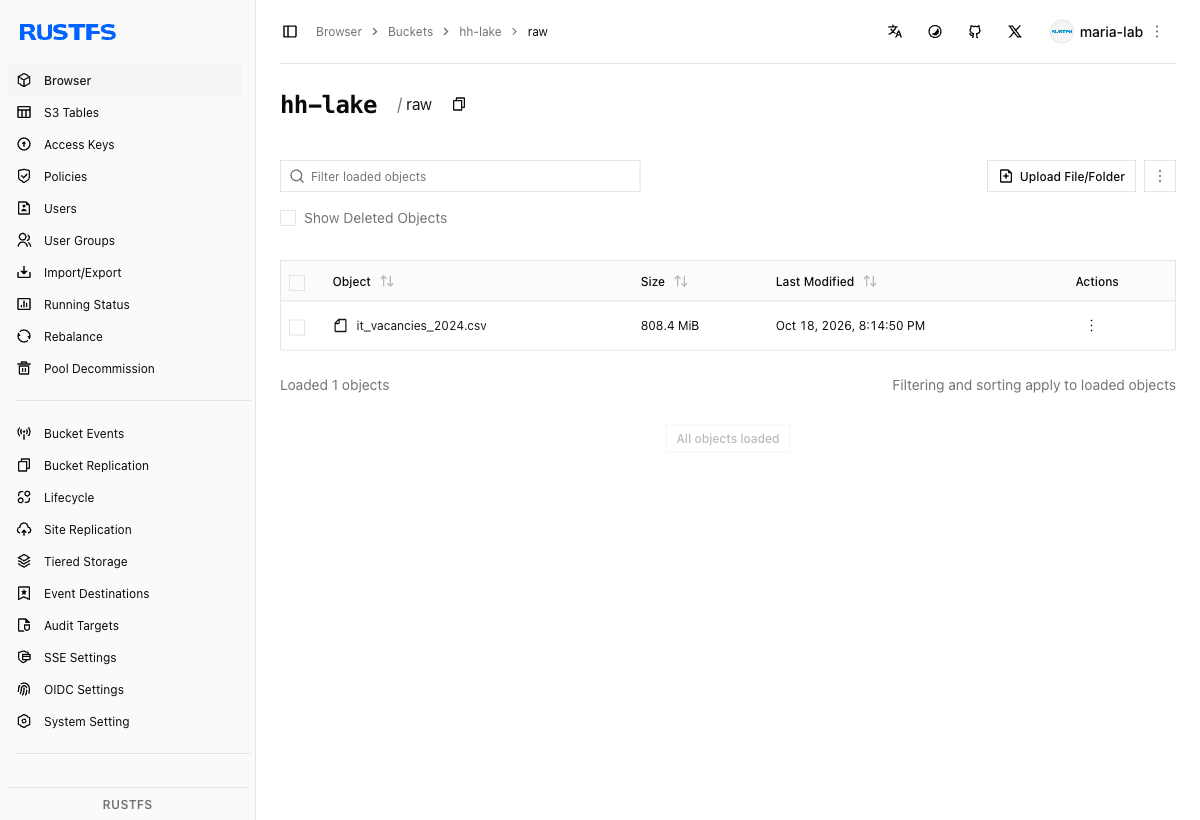
\includegraphics[width=\linewidth,trim=250bp 380bp 10bp 0bp,clip]{images/rustfs-raw.png}
\caption{Реальная консоль RustFS: исходный CSV в \texttt{hh-lake/raw}. Показана верхняя часть окна; размер в консоли округлён до МиБ.}
\end{figure}
\texttt{prepare.py} выполняет загрузку и контроль, \texttt{jobs.py} --- вычисления, \texttt{artifacts.py} --- сохранение результатов и подготовку Parquet. Порядок запуска расчётов приведён в разделе~\ref{sec:commands}.

\clearpage
\section{Собственная реализация MapReduce}
\texttt{boto3.get\_object} отдаёт поток \texttt{StreamingBody}. Адаптер с буфером 1~МиБ передаёт его в \texttt{csv.DictReader}; CSV с кавычками и переводами строк внутри полей разбирается как записи, а не строки текста. Файл целиком в память не загружается.

Чанк содержит 5\,000 исходных записей; всего получилось 46 чанков, последний --- 4\,388 записей. После разбора из 23 столбцов оставляются девять нужных. Mapper фильтрует вариант и для каждого набора размера $k=1,2,3$ выдаёт ключ \texttt{(регион, сочетание)} и частичную частоту со списком раскрытых зарплат. Вакансия добавляет к одному сочетанию не более единицы.
\begin{terminal}
skills = parse_skills(row['key_skills'])
for k in (1, 2, 3):
    for stack in itertools.combinations(skills, k):
        emit((scope, stack), (1, salary2))
\end{terminal}
Это сокращённая схема операции; исполняемый код находится в \texttt{jobs.py}. Частоты и значения зарплат предварительно объединяются внутри mapper. Reducer суммирует частоты, объединяет зарплатные наблюдения и вычисляет точную медиану. Медианы отдельных чанков не усредняются: такая операция в общем случае неверна.

Для параллельного режима применён \texttt{ProcessPoolExecutor} с четырьмя процессами. Одновременно ожидается не более восьми заданий. Чтение и CSV-разбор выполняет координатор; сериализация результатов, общий reducer и вывод JSON также создают последовательную часть. Это локальная реализация парадигмы MapReduce с чтением S3; кластер Hadoop в этих опытах не запускался.

Память чтения ограничена буфером и очередью чанков, однако reducer хранит все уникальные сочетания и зарплаты для точной медианы. Поэтому память всего расчёта не константна по объёму данных. Для больших объёмов потребуется разбиение reducer по ключу и внешняя сортировка/запись промежуточных результатов.

\subsection{Проверка отказа задания mapper}
В первом выполнении чанка №~2 намеренно выбрасывается исключение до фиксации результата. Координатор повторяет этот чанк; множество подтверждённых номеров защищает reducer от повторного зачёта.
\begin{terminal}
$ python jobs.py mapreduce --workers 4 --fault-chunk 2 \
    --config config.json --output results/fault-retry.json
mapper_failures: 1; committed_chunks: 46
matched_vacancies: 7993; combination_groups: 510189
elapsed_seconds: 7.982230916997651
\end{terminal}
Полный результат совпал с обычным запуском. Проверялся отказ вычислительного задания (исключение), а не аварийное завершение ОС-процесса, машины или S3-сервера. Отдельно четыре автоматических теста проверили фильтр Java/JavaScript, нормализацию, зарплаты, многострочный CSV и повтор задания на синтетическом тестовом объекте; все прошли.

\clearpage
\section{Независимый расчёт в DuckDB}\label{sec:sql}
DuckDB~1.5.6 читает тот же \texttt{s3://hh-lake/raw/it\_vacancies\_2024.csv} через расширение \texttt{httpfs}. Подключение настраивается временным \texttt{CREATE SECRET}: endpoint локального RustFS, \texttt{URL\_STYLE 'path'}, \texttt{USE\_SSL false}. Секрет не записывается в SQL-файл. Прямое чтение S3 и Parquet поддерживается DuckDB.

Фильтр SQL не использует Python-функцию \texttt{selected}; нормализация, генерация сочетаний и агрегация также написаны SQL-операциями.
\begin{terminal}
WHERE role = 'Программист, разработчик'
  AND (
    regexp_matches(coalesce(name, ''),
                   '(^|[^a-z])java([^a-z]|$)', 'i')
    OR list_contains(
      list_transform(
        string_split(coalesce(key_skills, ''), ';'),
        x -> lower(trim(x, chr(32)||chr(9)||chr(10)||chr(13)))
      ), 'java')
  )
\end{terminal}
\texttt{list\_distinct}, \texttt{list\_sort} и удаление пустых элементов задают такое же множество навыков. Во временной таблице \texttt{selected} сохраняются ID, регион, нормализованные навыки и удвоенная зарплата \texttt{salary2}. Представление \texttt{scoped} содержит общий срез и три региональных среза. Для пар используются индексы $i<j$, для троек --- $i<j<k$:
\begin{terminal}
SELECT scope, [skills[i],skills[j],skills[k]] AS combination,
       count(*), count(salary2), median(salary2)/2
FROM scoped,
     UNNEST(range(1, len(skills)+1)) a(i),
     UNNEST(range(i+1, len(skills)+1)) b(j),
     UNNEST(range(j+1, len(skills)+1)) c(k)
GROUP BY scope, combination;
\end{terminal}
Использована точная агрегатная \texttt{median}, а не приближённый квантиль. Воспроизводимый SQL со всеми вспомогательными таблицами и представлением сохранён в \texttt{results/reference-sql.sql}.
\begin{terminal}
$ python jobs.py duckdb --workers 4 --config config.json \
    --output results/reference-sql.json
matched_vacancies: 7993 combination_groups: 510189
\end{terminal}
Дополнительный pandas-baseline читает полный CSV в DataFrame, применяет Python-фильтр, материализует сочетания и выполняет \texttt{groupby}. Он нужен для сравнения ресурсов; независимая проверка обеспечена именно парой Python MapReduce / DuckDB SQL.

\clearpage
\section{Частоты, комбинаторный рост и верификация}
Для вакансии с $m$ различными навыками получается $m$ одиночных элементов, $\binom m2=m(m-1)/2$ пар и $\binom m3=m(m-1)(m-2)/6$ троек. Например, при $m=10$ это 10, 45 и 120 записей, а при $m=30$ --- 30, 435 и 4\,060. В данных есть 15 вакансий с 30 нормализованными навыками, которые одни дают 60\,900 вхождений троек.
\begin{table}[h!]
\centering\small
\caption{Число сочетаний по всему Java-сегменту, без дублирования региональных срезов.}
\begin{tabularx}{\linewidth}{rXrr}\toprule
$k$ & Уникальные стеки & Сумма частот & Проверка $\sum_v {m_v\choose k}$\\\midrule
1 & 2~031 & 42~604 & 42~604\\
2 & 34~529 & 184~684 & 184~684\\
3 & 249~480 & 690~362 & 690~362\\
\bottomrule\end{tabularx}
\end{table}

«Сумма частот» --- число вхождений до глобальной группировки; «уникальные стеки» --- число различных ключей после неё. Троек по вхождениям в 3,74 раза больше пар, по уникальным ключам --- в 7,23 раза. Разнообразие сочетаний повышает объём промежуточных данных и нагрузку на reducer, даже когда исходный файл читается одним проходом.

В сумме для общего среза 286\,040 групп; с тремя региональными срезами --- \textbf{510\,189}. Сравнивались не только три итоговых числа, но и полный упорядоченный список строк: регион, навыки, частота, число зарплат, точная медиана. Дополнительно сверены все ID выбранных вакансий, региональные итоги, число пустых списков и гистограмма числа навыков.
\begin{terminal}
$ python analyse.py
verified_files: 17
matched: 7993
groups: 510189
full_equality: true
\end{terminal}
Проверены независимый SQL-результат, результат с отказом mapper и все 15 файлов трёхкратных измерений. Численные поля совпали точно, без допуска округления. Контрольная SHA-256 канонического сравниваемого представления:
\begin{terminal}
9b30b39115c94adf5b74bfcec17036e3873
29f6f2be54520a029b8b5e16c43f0
\end{terminal}
Хеш дополняет полное сравнение полей. Исходный SHA-256 также совпал у исходного S3-объекта и потока чтения MapReduce; следовательно, расчёт действительно обработал весь CSV.

\clearpage
\section{Сохранение трёх размеров стека в S3}
Результат MapReduce сохранён в трёх Parquet-объектах. Поля: \texttt{region}, \texttt{skills} (список), \texttt{frequency}, \texttt{salary\_count}, \texttt{median\_salary\_rub}. Регион \texttt{\_\_ALL\_\_} обозначает общий срез. Число строк ниже включает также три региональных среза.
\begin{table}[h!]\centering\small
\caption{Объекты в \texttt{s3://hh-lake/results/java/}.}
\begin{tabularx}{\linewidth}{Xrrr}\toprule
Объект & $k$ & Строк & Байт\\\midrule
\texttt{java\_skills\_1.parquet} & 1 & 4\,303 & 32\,087\\
\texttt{java\_skills\_2.parquet} & 2 & 65\,659 & 274\,146\\
\texttt{java\_skills\_3.parquet} & 3 & 440\,227 & 2\,085\,588\\
\bottomrule\end{tabularx}\end{table}
\begin{terminal}
$ python artifacts.py store --config config.json \
    --result results/reference-mr.json --output results/stored
k=1: groups=4303   bytes=32087   HTTP=200
k=2: groups=65659  bytes=274146  HTTP=200
k=3: groups=440227 bytes=2085588 HTTP=200
local_SHA256 == downloaded_SHA256: true (all three)
\end{terminal}
Каждый объект прочитан обратно из RustFS; хеш скачанных байтов совпал с локальным. Полные хеши и HTTP-статусы находятся в \texttt{results/stored/s3-results.json}.
\begin{figure}[h!]
\centering
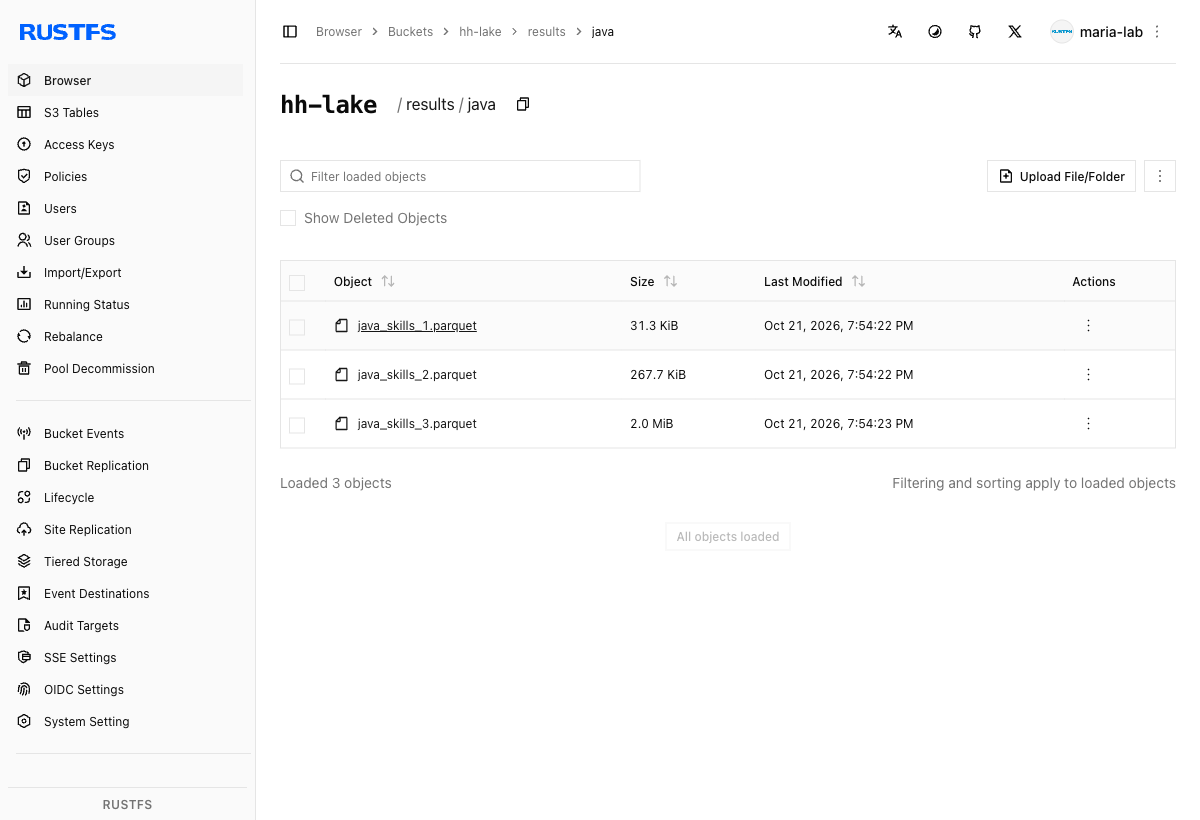
\includegraphics[width=\linewidth,trim=250bp 230bp 10bp 0bp,clip]{images/rustfs-results.png}
\caption{Реальный список результатов для $k=1,2,3$ в консоли RustFS.}
\end{figure}

\clearpage
\section{Профилирование времени и памяти}
Среда измерений: macOS~26.6.2, arm64, 12 логических CPU, 36~ГиБ RAM; Python~3.12.14, pandas~3.0.6, DuckDB~1.5.6. Каждый опыт запускается новым процессом. Выполнено по три попытки для пяти режимов; порядок режимов циклически сдвигается между попытками. Кэши ОС и RustFS прогреты, принудительно не очищались. Временные отметки и точные значения записаны в \texttt{results/benchmark.json}.

Wall time включает запуск и импорты клиента, чтение S3, фильтрацию, все три размера сочетаний, региональные срезы, медианы и сохранение полного JSON-результата. Паркетизация измеряется отдельно. Между опросами RSS задана пауза 10~мс; фактический интервал включает обход дерева процессов. Измеряется сумма RSS клиента и всех его дочерних процессов. Общие страницы могут учитываться повторно; процесс RustFS исключён из всех режимов. Это потребление дерева вычисления, а не уникально занятая физическая RAM всего компьютера.
\begin{table}[h!]
\centering\small
\caption{Все попытки профилирования; МиБ = $2^{20}$ байт.}
\begin{tabularx}{\linewidth}{Xrrr}\toprule
Подход & Попытка & Время, с & Пик RSS, МиБ\\\midrule
pandas, CSV & 1 & 28,794 & 3~099,1\\
pandas, CSV & 2 & 29,173 & 2~977,0\\
pandas, CSV & 3 & 30,615 & 2~878,2\\
MapReduce, 1 процесс & 1 & 8,919 & 434,7\\
MapReduce, 1 процесс & 2 & 10,210 & 413,5\\
MapReduce, 1 процесс & 3 & 8,757 & 412,1\\
MapReduce, 4 процесса & 1 & 8,555 & 491,6\\
MapReduce, 4 процесса & 2 & 11,171 & 472,5\\
MapReduce, 4 процесса & 3 & 8,385 & 469,0\\
DuckDB, CSV & 1 & 5,169 & 1~759,7\\
DuckDB, CSV & 2 & 9,860 & 1~608,1\\
DuckDB, CSV & 3 & 8,170 & 1~941,4\\
DuckDB, Parquet & 1 & 3,612 & 824,3\\
DuckDB, Parquet & 2 & 5,375 & 854,8\\
DuckDB, Parquet & 3 & 5,715 & 799,7\\
\bottomrule\end{tabularx}
\end{table}

Код профилирования: \texttt{benchmark.py}; запуск --- \texttt{python benchmark.py --attempts 3}. Во всех 15 попытках код выхода~0; предел 6~ГиБ, заданный профилировщиком для аварийного прекращения, не достигнут. В DuckDB задан лимит памяти оператора 2~ГБ: RSS процесса может быть выше из-за Python, библиотек и сериализации результата. Вариативность времени существенна, поэтому далее используется медиана, а не лучший запуск.

\clearpage
\section{Сравнение подходов и оптимизация}
\begin{table}[h!]
\centering\small
\caption{Медианы трёх попыток для каждого подхода.}
\begin{tabularx}{\linewidth}{Xrr}\toprule
Подход & Время, с & Пик RSS, МиБ\\\midrule
pandas, CSV & 29,173 & 2~977,0\\
MapReduce, 1 процесс & 8,919 & 413,5\\
MapReduce, 4 процесса & 8,555 & 472,5\\
DuckDB, CSV & 8,170 & 1~759,7\\
DuckDB, Parquet & 5,375 & 824,3\\
\bottomrule\end{tabularx}
\end{table}

\begin{figure}[h!]\centering
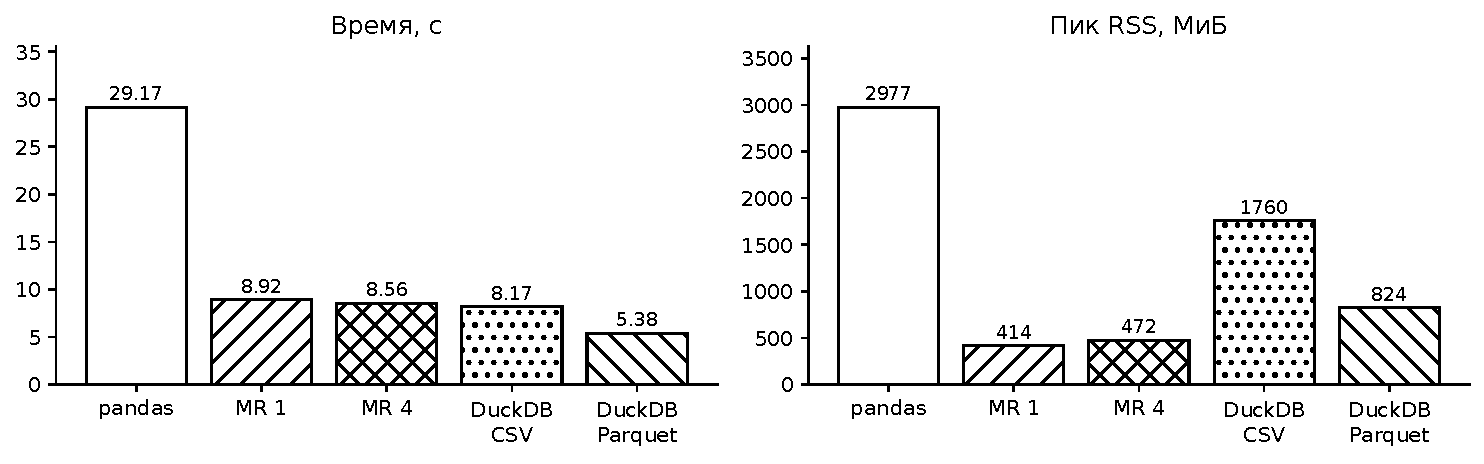
\includegraphics[width=\linewidth]{images/performance.pdf}
\caption{Медианы измеренного wall time и медианы пиков RSS; три попытки на режим.}
\end{figure}
pandas занимает около 2,91~ГиБ: в памяти сосуществуют полный CSV со столбцами описаний, промежуточные сочетания и группировка. Однопроцессный потоковый MapReduce использует в 7,20 раза меньше RSS и выполняется в 3,27 раза быстрее. Четыре процесса дают лишь около 4,1\% выигрыша по медиане времени против одного, увеличивая медиану RSS на 14,3\%; расходы на передачу данных и последовательные стадии существенны.

\subsection{Бонус: проекция и колоночный формат}
\texttt{artifacts.py optimize} один раз читает полный CSV из S3, оставляет девять используемых столбцов \emph{для всех} 229\,388 строк и создаёт Parquet с ZSTD. Вариант Java заранее не фильтруется. Полученный объект \texttt{optimized/it\_vacancies\_core.parquet} имеет размер 7\,365\,457 байт; подготовка, включая загрузку результата в S3, заняла 1,553~с. Уменьшение объёма в 115,08 раза связано одновременно с удалением описаний и остальных ненужных полей и с кодированием Parquet; приписывать всё сжатию одинаковых данных было бы неверно.

При том же SQL DuckDB медиана времени снизилась с 8,170 до 5,375~с: ускорение 1,52 раза, экономия времени 34,2\%. Медиана пика RSS снизилась с 1\,759,7 до 824,3~МиБ, то есть на 53,2\%. Полный результат совпал во всех попытках. Разовая подготовка окупается при
\[
q>\frac{T_{prep}}{T_{CSV}-T_{Parquet}}
=\frac{1{,}553}{8{,}170-5{,}375}=0{,}56.
\]
Для этого конкретного прогона даже один повторный расчёт вместе с подготовкой укладывается примерно в 6,93~с. Это оценка по измеренным медианам и одному времени подготовки, а не гарантия для любого оборудования или холодного хранилища.

\clearpage
\section{Зарплаты: правила сопоставления}
Для анализа используются только \texttt{currency='RUR'} и \texttt{gross=false}: раскрытые суммы «на руки» в рублях. Другие валюты, зарплаты до налога и неизвестный признак gross исключаются из медиан, но сохраняются в частотах навыков. Если заданы две положительные границы, берётся их полусумма; если одна --- она. Нулевые, отрицательные и некорректные значения не используются. Конвертация валют и расчёт налога не проводились.

Всего сопоставимая зарплата найдена у \textbf{1\,360 из 7\,993 вакансий} (17,0\%); общая медиана --- \textbf{180\,000 руб.} Используется точная медиана индивидуальных оценок вакансий. В Python суммы хранятся удвоенными целыми числами; после медианы деление на два сохраняет точность полусумм.
\begin{table}[h!]
\centering\small
\caption{Наиболее частые навыки; медиана только по раскрытым зарплатам net в рублях.}
\begin{tabularx}{\linewidth}{Xrrr}\toprule
Навык & Частота $F$ & Зарплат $n$ & Медиана, тыс. руб.\\\midrule
java & 5~629 & 1~102 & 175,0\\
spring framework & 2~177 & 336 & 215,0\\
postgresql & 2~036 & 359 & 200,0\\
sql & 1~681 & 380 & 180,0\\
git & 1~517 & 384 & 185,0\\
kotlin & 1~154 & 255 & 200,0\\
spring boot & 1~048 & 194 & 220,0\\
kafka & 1~046 & 136 & 250,0\\
docker & 836 & 170 & 225,0\\
ооп & 729 & 128 & 130,0\\
\bottomrule\end{tabularx}
\end{table}

Частота Java (5\,629) меньше числа вакансий сегмента: часть отобрана по названию, включая вакансии без списка навыков. Группы пересекаются и не являются взаимно исключающими категориями.

\subsection{База для дополнительного навыка}
Для пары $C=\{a,b\}$ база $B$ --- более частый одиночный навык, частота считается по всем вакансиям сегмента. Для тройки база --- наиболее частая из её трёх пар. При равенстве частот используется лексикографический порядок; не выбирается база с удобной медианой. В сравнении остаются только сочетания с $n_C\ge20$ раскрытыми сопоставимыми зарплатами.
\[
\Delta=M_C-M_B,\qquad
L=100\%\left(\frac{M_C}{M_B}-1\right).
\]
Рейтинг упорядочен по $L$, при равенстве --- по числу зарплат и названию. $F$ означает число вакансий со стеком, $n$ --- число зарплат, $M$ --- медиану; $C=B\cup\{x\}$. Базовая группа содержит расширенную, поэтому это описательная разница вложенных выборок, не причинная оценка дохода от освоения навыка.

\clearpage
\section{Пары с ростом и снижением медианы}
Порог $n_C\ge20$ прошли 293 пары. В таблице приведены первые три положительные и первые три отрицательные ассоциации по относительному изменению. В каждой строке показаны частота и зарплатная поддержка обеих групп, в том числе базовой.
\begin{table}[h!]
\centering\small
\caption{Три наибольших роста и три снижения относительной медианы: пары.}
\begin{tabularx}{\linewidth}{>{\raggedright\arraybackslash}Xrrrr}\toprule
База $B$; ниже $+x$ & $F_B\to F_C$ & $n_B\to n_C$ & $M_B\to M_C$, тыс. руб. & $\Delta$, тыс. руб.\\\midrule
java\newline $+\,$microservices & 5~629$\to$116 & 1~102$\to$26 & 175,00$\to$300,00 & +125,00\newline (+71,4\%)\\
java\newline $+\,$nosql & 5~629$\to$84 & 1~102$\to$23 & 175,00$\to$295,00 & +120,00\newline (+68,6\%)\\
java\newline $+\,$rabbitmq & 5~629$\to$430 & 1~102$\to$68 & 175,00$\to$280,00 & +105,00\newline (+60,0\%)\\
sql\newline $+\,$c\# & 1~681$\to$82 & 380$\to$21 & 180,00$\to$77,28 & -102,72\newline (-57,1\%)\\
java\newline $+\,$обучение и развитие & 5~629$\to$56 & 1~102$\to$27 & 175,00$\to$75,60 & -99,40\newline (-56,8\%)\\
java\newline $+\,$c\# & 5~629$\to$192 & 1~102$\to$66 & 175,00$\to$78,64 & -96,36\newline (-55,1\%)\\
\bottomrule\end{tabularx}
\end{table}

У пары Java + microservices медиана 300~тыс. руб. против 175~тыс. у Java: разница 125~тыс. руб., или 71,4\%. Однако зарплаты раскрыты только у 26 из 116 вакансий пары; без учёта стажа, уровня позиции, работодателя и региона это не оценка рыночной надбавки за один навык. Java + NoSQL и Java + RabbitMQ также связаны с более высокой медианой; вероятная интерпретация --- более сложные backend-задачи, но отдельная проверка этой гипотезы не проводилась.

Низкая медиана C\# + SQL (77\,280 руб.) не означает, что C\# уменьшает зарплату Java-разработчика. В отобранном сегменте встречаются смешанные требования и младшие позиции. В контрольной выборке исходных названий обнаружены \emph{Trainee developer (Salesforce)} с 20~тыс. руб., \emph{Инженер-программист (Junior SQL developer)} с 49,2~тыс. руб., стажёры и преподаватели программирования. Примеры сохранены в \texttt{results/coverage.json}. Они объясняют возможность такого состава группы, но не доказывают причину всей разницы.

Для Java + «обучение и развитие» медиана 75\,600 руб. при $n=27$. Результат совместим с присутствием учебных и начальных позиций. Использовать эту ассоциацию как рекомендацию отказаться от обучения нельзя. Все ставки относятся к раскрывающей зарплаты части датасета 2024 года; публикация зарплат неслучайна, а порог 20 не заменяет доверительный интервал.

Полный рейтинг всех прошедших порог пар находится в \path{results/salary_associations_2.csv}; исходные группировки без порога сохранены в Parquet.

\clearpage
\section{Тройки с ростом и снижением медианы}
Порог поддержки прошла 371 тройка. База каждой строки выбрана по максимальной частоте пары, а не одиночного навыка и не минимальной зарплате. Поэтому процентный рост тройки нельзя напрямую сравнивать с ростом пары как одинаковую «надбавку».
\begin{table}[h!]
\centering\small
\caption{Три наибольших роста и три снижения относительной медианы: тройки.}
\begin{tabularx}{\linewidth}{>{\raggedright\arraybackslash}Xrrrr}\toprule
База $B$; ниже $+x$ & $F_B\to F_C$ & $n_B\to n_C$ & $M_B\to M_C$, тыс. руб. & $\Delta$, тыс. руб.\\\midrule
java + javascript\newline $+\,$typescript & 518$\to$69 & 167$\to$25 & 100,00$\to$185,00 & +85,00\newline (+85,0\%)\\
java + sql\newline $+\,$spring & 1~600$\to$135 & 353$\to$23 & 175,00$\to$300,00 & +125,00\newline (+71,4\%)\\
java + sql\newline $+\,$rabbitmq & 1~600$\to$109 & 353$\to$30 & 175,00$\to$270,00 & +95,00\newline (+54,3\%)\\
java + sql\newline $+\,$c\# & 1~600$\to$82 & 353$\to$21 & 175,00$\to$77,28 & -97,72\newline (-55,8\%)\\
html + java\newline $+\,$c\# & 307$\to$49 & 106$\to$22 & 100,00$\to$50,00 & -50,00\newline (-50,0\%)\\
java + kotlin\newline $+\,$mvvm & 1~133$\to$71 & 251$\to$22 & 200,00$\to$100,00 & -100,00\newline (-50,0\%)\\
\bottomrule\end{tabularx}
\end{table}

Самая большая относительная разница получена при добавлении TypeScript к Java + JavaScript: 185~тыс. руб. вместо 100~тыс., рост 85\% ($n_C=25$). Стек содержит Java по правилу варианта; сочетание с JavaScript не делает его вакансией, отобранной только по JavaScript. База из Java + JavaScript встречается 518 раз и действительно чаще двух других пар этой тройки.

Для Java + SQL + Spring база Java + SQL имеет частоту 1\,600 и медиану 175~тыс. руб.; тройка --- 300~тыс. руб. при 23 зарплатах. \texttt{spring} здесь не объединён со \texttt{spring framework}; это ещё одна причина не трактовать сравнение как универсальную оценку технологии.

Снижения на 50--55,8\% наблюдаются для показанных смешанных стеков и Java + Kotlin + MVVM. Для последнего медиана падает с 200 до 100~тыс. руб. при $n_C=22$, однако причину без контроля уровней позиций и географии установить нельзя. Разные исходные группы и состав раскрывающих зарплату работодателей способны менять медиану сильнее, чем сам дополнительный навык.

Положительные и отрицательные строки --- одинаково важные результаты: они показывают ограничение простого сравнения медиан. Это инструмент поиска гипотез и проверки качества сегмента, а не причинная модель заработка. Полный рейтинг находится в \path{results/salary_associations_3.csv}.

\clearpage
\section{Региональный анализ}
Выбраны Москва, Санкт-Петербург и Екатеринбург. Объём последнего меньше, но есть 48 сопоставимых зарплат, что позволяет описательное сравнение. Регион берётся буквально из \texttt{area}; область, удалённая работа и агломерация отдельно не объединяются. Подсчёт вакансий и базовая медиана не зависят от заполненности навыков.
\begin{table}[h!]
\centering\small
\caption{Региональная таблица 1: все вакансии варианта, включая вакансии без навыков.}
\begin{tabularx}{\linewidth}{>{\raggedright\arraybackslash}Xrrrrr}\toprule
Регион & Вакансий & Без навыков & Зарплат $n$ & Доля $n$, \% & Медиана, тыс. руб.\\\midrule
Москва & 3~831 & 1~150 & 563 & 14,7 & 225,0\\
Санкт-Петербург & 1~058 & 286 & 214 & 20,2 & 200,0\\
Екатеринбург & 304 & 78 & 48 & 15,8 & 130,0\\
\bottomrule\end{tabularx}
\end{table}

Москва даёт в 3,62 раза больше вакансий, чем Санкт-Петербург, но медиана выше на 12,5\%, а не пропорционально объёму рынка. Относительно Екатеринбурга московская медиана выше на 73,1\%. У Санкт-Петербурга наиболее высокая доля раскрытых net-зарплат в рублях: 20,2\% против 14,7\% в Москве; сравнение медиан относится к разным по полноте подвыборкам.

\begin{table}[h!]
\centering\small
\caption{Региональная таблица 2: самый частый стек каждой длины. Доля от всех вакансий региона.}
\begin{tabularx}{\linewidth}{lr>{\raggedright\arraybackslash}Xrrrr}\toprule
Регион & $k$ & Навыки & $F$ & Доля, \% & $n$ & Медиана, тыс. руб.\\\midrule
Москва & 1 & java & 2~493 & 65,1 & 433 & 230,0\\
Москва & 2 & java + spring framework & 943 & 24,6 & 153 & 250,0\\
Москва & 3 & java + postgresql + spring framework & 457 & 11,9 & 79 & 250,0\\
СПб & 1 & java & 732 & 69,2 & 178 & 187,5\\
СПб & 2 & java + spring framework & 266 & 25,1 & 56 & 240,0\\
СПб & 3 & java + postgresql + spring framework & 145 & 13,7 & 29 & 230,0\\
Екатеринбург & 1 & java & 208 & 68,4 & 40 & 142,5\\
Екатеринбург & 2 & java + postgresql & 73 & 24,0 & 12 & 175,0\\
Екатеринбург & 3 & java + postgresql + spring framework & 40 & 13,2 & 7 & 130,0\\
\bottomrule\end{tabularx}
\end{table}

При равенстве частот лидер выбирается лексикографически. $F$ и доля в таблице~\thetable{} рассчитаны по всем вакансиям региона, $n$ и медиана --- по его зарплатной подвыборке. Стек размера $k$ может входить в вакансию с большим числом навыков; таблица показывает включение сочетания, а не точное равенство полного списка навыков.

\clearpage
\subsection*{Наблюдения по регионам}
Самый частый отдельный навык во всех трёх регионах --- Java. При этом доли от всех вакансий близки: 65,1\% в Москве, 69,2\% в Санкт-Петербурге и 68,4\% в Екатеринбурге. Учитывать вакансии без навыков существенно: их соответственно 1\,150, 286 и 78; исключение изменило бы знаменатели и искусственно увеличило доли.

В Москве и Санкт-Петербурге лидирует пара Java + Spring Framework (943 и 266 вакансий), в Екатеринбурге --- Java + PostgreSQL (73). Это различие частот в данной выгрузке, а не доказательство различий технологий всех компаний региона. Лидирующая тройка во всех случаях одна: Java + PostgreSQL + Spring Framework.

У этой тройки медианы 250, 230 и 130~тыс. руб. соответственно. Для Екатеринбурга медиана основана всего на семи зарплатах. Она приведена, чтобы не скрывать малую поддержку, но делать из неё уверенный вывод о надбавке за стек нельзя. У Москвы для той же тройки 79 зарплат, у Санкт-Петербурга --- 29. Следующий шаг для более надёжного сравнения --- сопоставить опыт, работодателей, тип занятости и периоды публикации, а затем оценить неопределённость.

\section{Выводы и выбор инструмента}
Собственный MapReduce и независимо записанный DuckDB SQL дали полное совпадение частот и медиан, включая региональные срезы. Повтор отказавшего задания не изменил результат. Все три размера стека сохранены в \texttt{hh-lake}; комбинаторный рост подтверждён как по уникальным группам, так и по сумме вхождений.

Для повторного анализа этого файла я выбрала бы \textbf{RustFS + Parquet + DuckDB}: медиана 5,38~с и 824~МиБ RSS, короткая проверяемая SQL-логика и удобное хранение результатов в S3. CSV полезен для обмена и первоначальной загрузки, но не для регулярного чтения длинных неиспользуемых описаний. pandas подходит для небольших выборок и исследования данных; его наивная реализация здесь затрачивает 29,17~с и около 2,91~ГиБ RSS.

Потоковый MapReduce полезен, когда нужен явный контроль обработки чанков, повторов и частичных агрегатов: медиана пика RSS однопроцессного режима составляет 413,5~МиБ. Его reducer всё ещё ограничен памятью одной машины. Для объёмов, которые не помещаются в RAM и требуют распределённого исполнения, понадобится отдельная архитектура с несколькими узлами, распределённым shuffle и хранением промежуточных результатов. Работоспособность и ресурсные характеристики такой системы на 24~ГБ этой лабораторной не измерялись.

Зарплатные ассоциации требуют осторожности: раскрыты лишь 17,0\% сопоставимых зарплат; группы пересекаются, а исходные названия навыков неоднородны. Рассчитанные медианы позволяют сформулировать гипотезы о сегментах рынка, но не обещать персональную прибавку от изучения технологии.

\clearpage
\section{Воспроизводимость и состав материалов}\label{sec:commands}
Исходный код, PDF, LaTeX, реальные снимки консоли и метрики профилирования подготовлены для репозитория
\begin{center}
\url{https://github.com/maryshirk/mapreduce-java-vacancies-2024}
\end{center}
Основная последовательность команд после настройки RustFS и локальных ключей:
\begin{terminal}
python prepare.py --source-file it_vacancies_2024.csv \
  --output evidence/input.json
python jobs.py mapreduce --workers 1 --config config.json \
  --output results/reference-mr.json
python jobs.py duckdb --workers 4 --config config.json \
  --output results/reference-sql.json
python jobs.py mapreduce --workers 4 --fault-chunk 2 \
  --config config.json --output results/fault-retry.json
python artifacts.py optimize --output evidence/parquet-prepare.json
python benchmark.py --attempts 3
python analyse.py
python inspect_data.py
python artifacts.py store --output results/stored
python -m unittest -v test_jobs.py
\end{terminal}
\texttt{requirements.txt} фиксирует версии. В GitHub публикуются программы, отчёт, иллюстрации и метрики времени и памяти; исходный CSV, подробные журналы и производные таблицы туда не загружаются. Компактные итоговые таблицы, полный SQL, контрольные хеши, журналы и Parquet-результаты приложены в локальном архиве материалов. Большие промежуточные JSON всех попыток создаются командами. В локальной копии журналов абсолютный корень домашнего каталога сокращён до \texttt{<project>} для приватности; вычисленные числа не изменены. В отчёте длинные JSON-выводы сокращены до полей, относящихся к проверке.

\end{document}
